\subsection{Graphene and hydrogen honeycomb lattice}
\label{subsection:graphene}
Our third example highlights the role of the high energy 
degrees of freedom not present in the low energy description 
but which are instrumental in renormalizing the effective interactions. 
We demonstrate this by considering the case of graphene, and by 
comparing it to artificially constructed counterparts without the high energy electrons. 
Although many electronic properties of graphene can be adequately 
described by a noninteracting tight-binding model of $\pi$ electrons~\cite{Castro2009}, 
electron-electron interactions are crucial for explaining 
a wide range of phenomena observed in experiments~\cite{Kotov2012}. 
In particular, electron screening from $\sigma$ bonding renormalizes 
the low energy plasmon frequency of the $\pi$ electrons~\cite{Zheng2016}. In fact, 
without the $\sigma$ electrons, a system of $\pi$ electrons with bare Coulomb interactions has been shown \lucas{by whom? and why do we care that people argued it?} \HHZ{I changed the word "argue" to "shown". "by whom" is answered in the citations. Also, we do not care  that people argued it, but we care the fact because it is directly related to our downfolding models. I added an extra sentence to strengthen this point} to be an 
insulator instead of a semimetal~\cite{DrutPRL2009, DrutPRB2009,  Smith2014, Zheng2016}. 
Using DMD, we demonstrate how the screening effect of $\sigma$ electrons is manifested in the low energy effective model of graphene. 

In order to disentangle the screening effect of $\sigma$ electrons from the bare interactions 
between $\pi$ electrons, we apply DMD to three different systems, graphene, $\pi$-only graphene, and a honeycomb lattice of hydrogen atoms.  
In the $\pi$-only graphene, the 
$\sigma$ electrons are replaced with a static constant negative charge background. 
The role of $\sigma$ electrons is then clarified by comparing the effective model Hamiltonians of these two systems. 
The hydrogen system we study has the same lattice constant $a=2.46$\AA~as graphene, 
which has a similar Dirac cone dispersion as graphene~\cite{Zheng2016}. 

By constructing the one-body space by Wannier localizing Kohn-Sham orbitals obtained from DFT calculations (see Fig.~\ref{fig:honeycomb_wan}), 
we verify that the low energy degrees of freedom correspond to the $\pi$ orbitals in graphene and 
its $\pi$-only system and $s$ orbitals in hydrogen; these enter the effective one-band Hubbard model description in Eq.~\eqref{eq:oneband}. 
Due to the vanishing density of states at the Fermi level, the Coulomb interaction remains long-ranged, 
in contrast to usual metals where the formation of electron-hole pairs screens the interactions strongly~\cite{Zheng2016}. 
However, for certain aspects, the long ranged part can be considered as renormalizing the 
onsite Coulomb interaction $U$ at low energy~\cite{Schuler2013, Changlani2015}. 
%Therefore, we expect that one-band Hubbard model is a reasonable description of the low energy physics. 
\lucas{Last sentence is not well-supported. In fact we know it has deficiencies and said so in our 2015 paper.}  \HHZ{I removed the last sentence.}

\begin{figure}
\centering
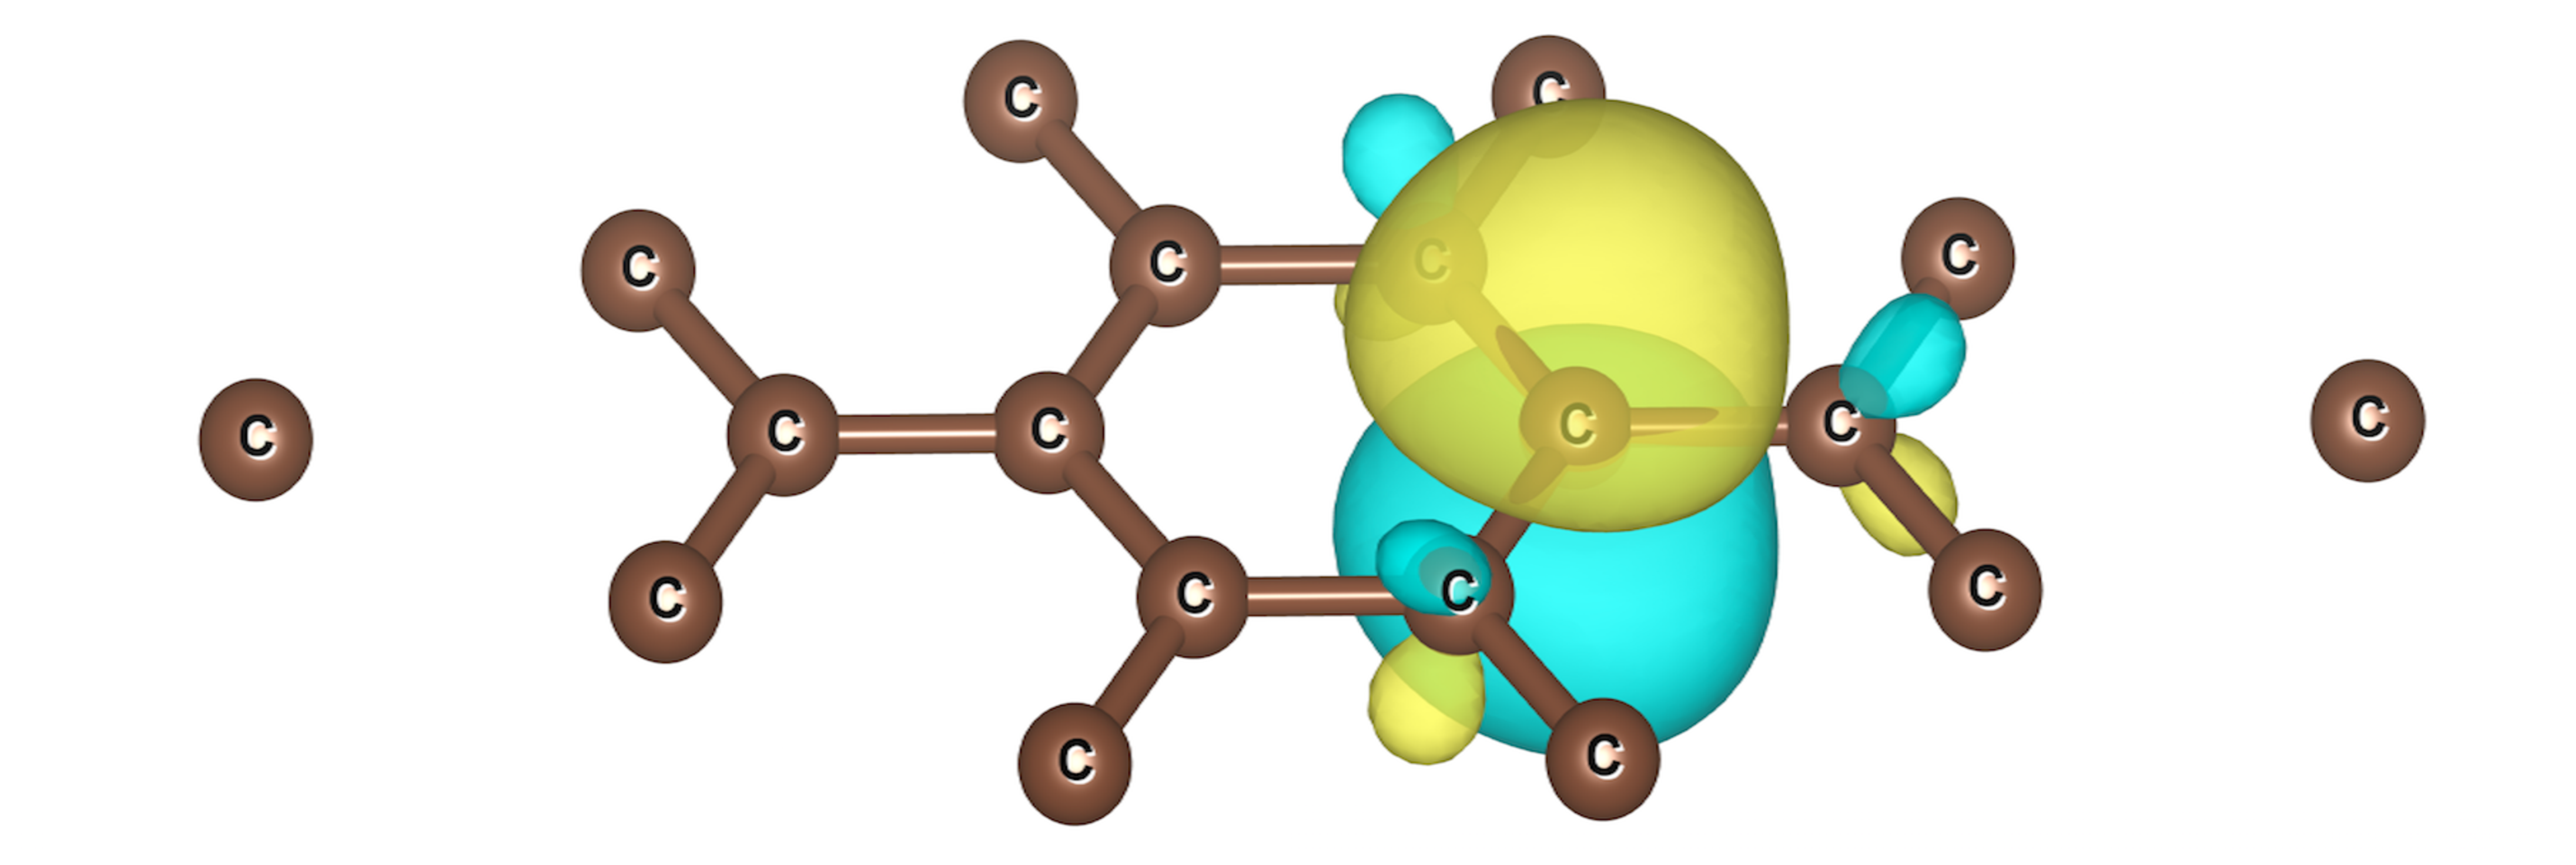
\includegraphics[width=0.40\textwidth]{./Figures/c_pi.eps}
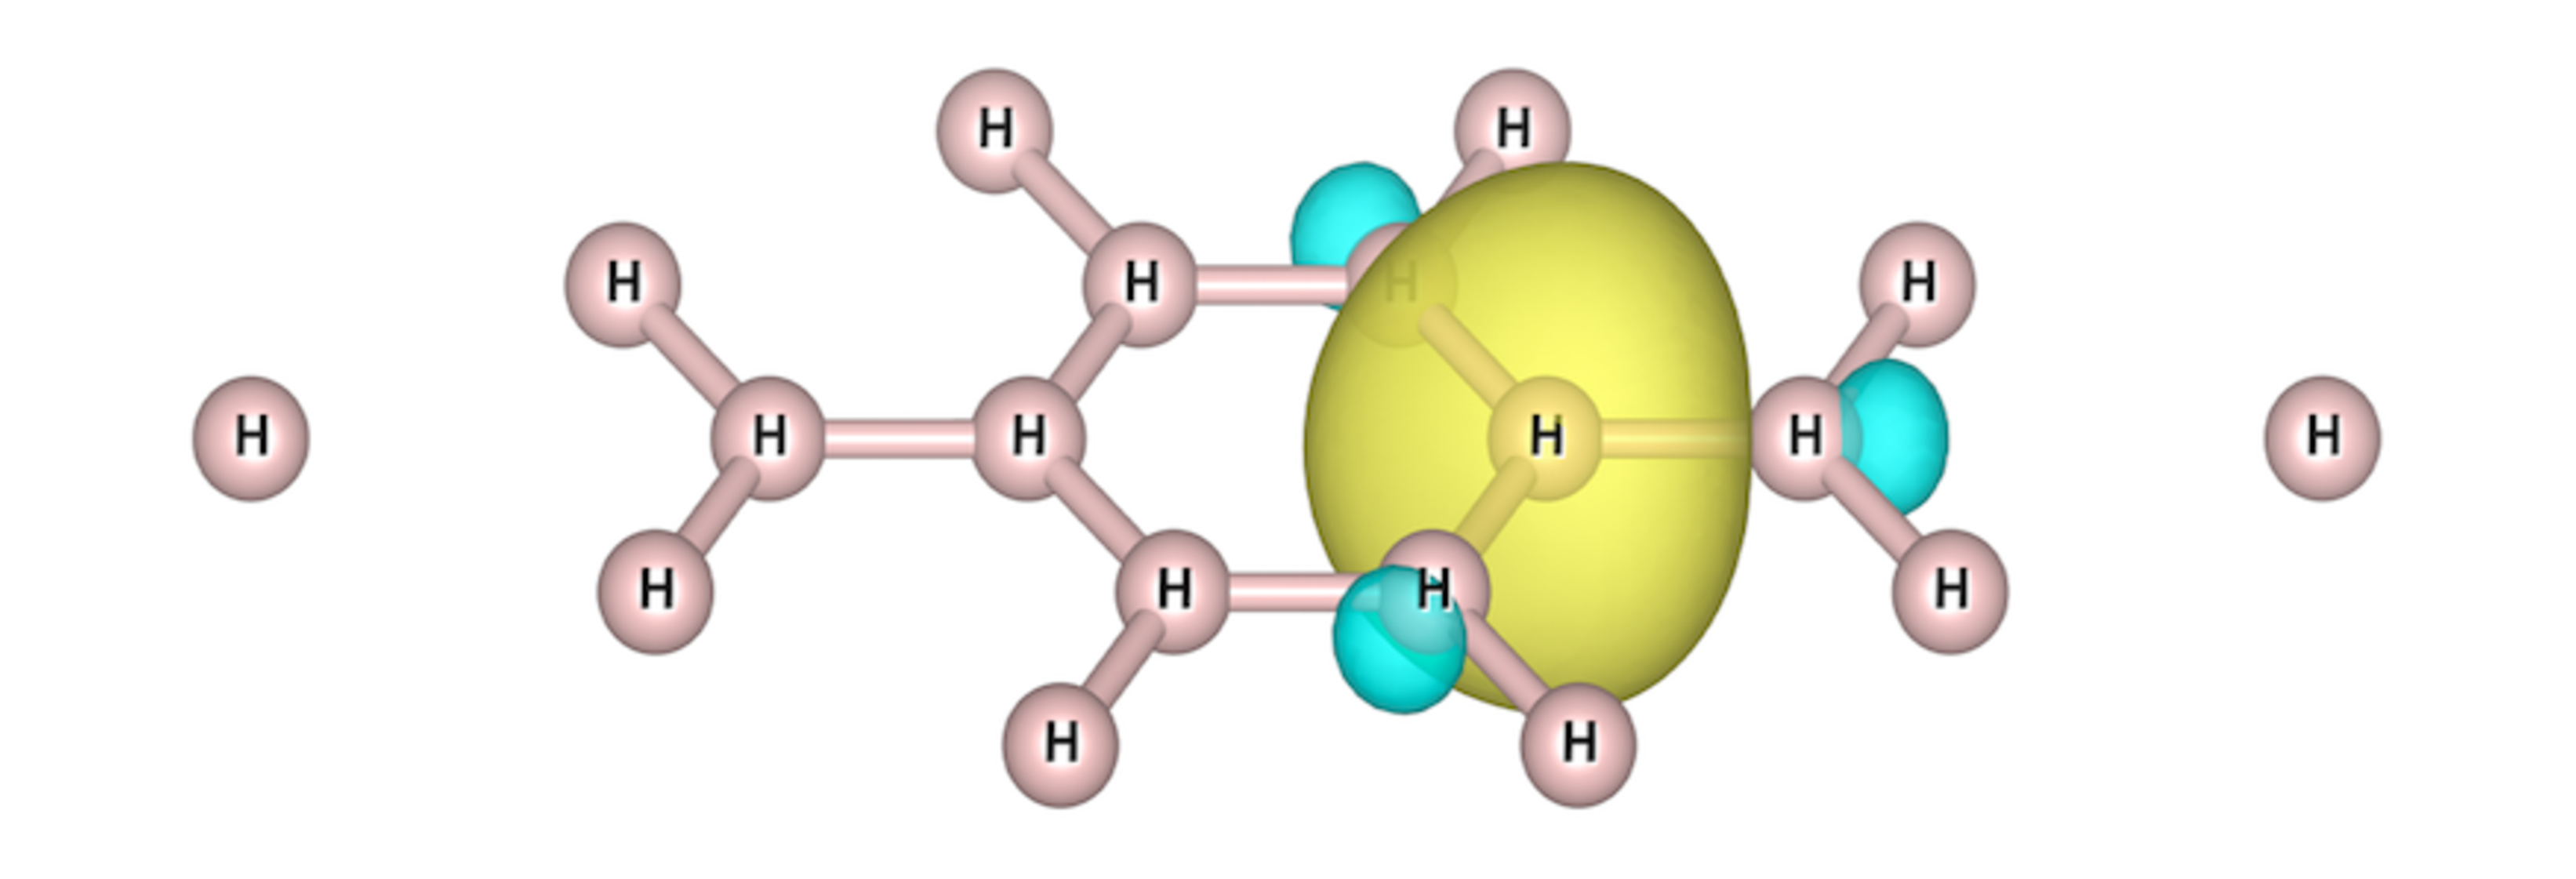
\includegraphics[width=0.40\textwidth]{./Figures/h_wan.eps}
\caption{Wannier orbitals constructed from Kohn-Sham orbitals: (A) graphene $\pi$ orbital; (B) hydrogen $s$ orbital. \lucas{Need some kind of titles to differentiate the graphs. $E[\Psi]$ versus $E_{eff}[\Psi]$ }\HHZ{I assume you meant next figure.}}
\label{fig:honeycomb_wan}
\end{figure}

To estimate the one-band Hubbard parameters, we used the DMD method using a set of 50 Slater-Jastrow wave functions that correspond 
to the electron-hole excitations within the $\pi$ channel for the graphene systems 
or $s$ channel for the hydrogen system. In particular, for graphene, 
the Slater-Jastrow wave functions are constructed from occupied $\sigma$ bands and occupied $\pi$ bands, whereas for $\pi$-only 
graphene, Slater-Jastrow wave functions constructed from occupied $\pi$ Kohn-Sham orbitals of graphene. The \textit{ab-initio} simulations 
were performed on a $3\times3$ cell (32 carbons or hydrogens) and the energy and RDMs of these wave functions were
evaluated with VMC. \footnote{We expect further renormalizations in the corresponding DMC calculations~\cite{Changlani2015}, 
but we do not explore that aspect here.\lucas{This is vague. Why should someone believe your results?} } The error bars on our downfolded parameters are estimated using the jackknife method.\lucas{citation} 
The results from our calculations are summarized in %Table~\ref{tab:grpheffm} 
Figure~\ref{fig:ne_aidmd_gh}.% shows the quality of the fits for the three systems.

%\begin{table}[ht]
%\centering
%\caption{Downfolding parameters for graphene and hydrogen.}
%\begin{tabular}{|c|c|c|c|}
%\hline
%Parameters [eV] & $\;\;\;\;$ graphene $\;\;\;$ & $\pi$-only graphene & $\;\;\;$hydrogen$\;\;\;$ \\
%\hline
%\hline
%$t$ & 3.61(1) & 2.99(1) & 3.73(1)\\
%$U$ & 7.16(3) & 14.8(2) & 9.47(5)\\
%\hline
%\end{tabular}

%\label{tab:grpheffm}
%\end{table} 

\begin{figure}
\centering
  \begin{tabular}{@{}p{0.95\linewidth}@{\quad}p{\linewidth}@{}}
    \subfigimg[clip, width=0.325\linewidth]{(A)}{./Figures/grp_all_tu.eps}
    \subfigimg[clip, width=0.325\linewidth]{(B)}{./Figures/grp_pi_tu.eps}
    \subfigimg[clip, width=0.325\linewidth]{(C)}{./Figures/h_tu.eps}
    \end{tabular}
\caption{Comparison of \textit{ab initio} (x-axis) and fitted energies (y-axis) of the 3$\times$3 periodic unit cell of graphene and hydrogen lattice: (A) graphene; (B) $\pi$-only graphene; (C) hydrogen lattice.}\label{fig:ne_aidmd_gh}
\end{figure}

We find that the one-band Hubbard model describes graphene and hydrogen very well, as is seen from the fact that $R^2$ is closed to 1 for the fittings. \lucas{$R^2$ is a better supporter of this statement.} \HHZ{$R^2$ now is included in the plot.} of the predicted energies; our fits are shown in Figure~\ref{fig:ne_aidmd_gh}
For both graphene and hydrogen, $U/t$ is smaller than the critical value of the 
semimetal-insulator transition $(U/t)_c \approx 3.8$ for the honeycomb lattice~\cite{Sorella2012}, 
which is consistent with both systems being semimetals. The two systems indeed have similar hopping constant $t$, 
consistent with the fact that they have similar Fermi velocities at the Dirac point. However, 
the difference in their high energy structure manifests itself as different renormalizated electron-electrons interactions, 
explaining the difference in $U$. Most prominently, the $\pi$-only system has much larger $U/t$ ($\sim4.9$) compared to graphene, 
which is large enough to push it into the insulating (antiferromagnetic) phase. %of the honeycomb lattice Hubbard model. 
Another important difference, which matches with our physical intuition,\lucas{how so?} \HHZ{this is explained in the next sentence.} is that graphene has larger $t$ than $\pi$-only graphene. 
We attribute this to the $\sigma$ electrons pushing $\pi$ electrons away from the ions through exchange-correlation interactions, 
which makes it easier for the $\pi$ electrons to hop to nearby sites. 
Thus, downfolding shows the clear significance of $\sigma$ electrons in renormalizing the effective onsite interactions of the $\pi$ orbitals. 
The $\sigma$ electrons change \textit{both} $t$ and $U$, making graphene a weakly interacting semimetal instead of an insulator.
